% Options for packages loaded elsewhere
\PassOptionsToPackage{unicode}{hyperref}
\PassOptionsToPackage{hyphens}{url}
%
\documentclass[
]{article}
\usepackage{amsmath,amssymb}
\usepackage{iftex}
\ifPDFTeX
  \usepackage[T1]{fontenc}
  \usepackage[utf8]{inputenc}
  \usepackage{textcomp} % provide euro and other symbols
\else % if luatex or xetex
  \usepackage{unicode-math} % this also loads fontspec
  \defaultfontfeatures{Scale=MatchLowercase}
  \defaultfontfeatures[\rmfamily]{Ligatures=TeX,Scale=1}
\fi
\usepackage{lmodern}
\ifPDFTeX\else
  % xetex/luatex font selection
\fi
% Use upquote if available, for straight quotes in verbatim environments
\IfFileExists{upquote.sty}{\usepackage{upquote}}{}
\IfFileExists{microtype.sty}{% use microtype if available
  \usepackage[]{microtype}
  \UseMicrotypeSet[protrusion]{basicmath} % disable protrusion for tt fonts
}{}
\makeatletter
\@ifundefined{KOMAClassName}{% if non-KOMA class
  \IfFileExists{parskip.sty}{%
    \usepackage{parskip}
  }{% else
    \setlength{\parindent}{0pt}
    \setlength{\parskip}{6pt plus 2pt minus 1pt}}
}{% if KOMA class
  \KOMAoptions{parskip=half}}
\makeatother
\usepackage{xcolor}
\usepackage[margin=1in]{geometry}
\usepackage{color}
\usepackage{fancyvrb}
\newcommand{\VerbBar}{|}
\newcommand{\VERB}{\Verb[commandchars=\\\{\}]}
\DefineVerbatimEnvironment{Highlighting}{Verbatim}{commandchars=\\\{\}}
% Add ',fontsize=\small' for more characters per line
\usepackage{framed}
\definecolor{shadecolor}{RGB}{248,248,248}
\newenvironment{Shaded}{\begin{snugshade}}{\end{snugshade}}
\newcommand{\AlertTok}[1]{\textcolor[rgb]{0.94,0.16,0.16}{#1}}
\newcommand{\AnnotationTok}[1]{\textcolor[rgb]{0.56,0.35,0.01}{\textbf{\textit{#1}}}}
\newcommand{\AttributeTok}[1]{\textcolor[rgb]{0.13,0.29,0.53}{#1}}
\newcommand{\BaseNTok}[1]{\textcolor[rgb]{0.00,0.00,0.81}{#1}}
\newcommand{\BuiltInTok}[1]{#1}
\newcommand{\CharTok}[1]{\textcolor[rgb]{0.31,0.60,0.02}{#1}}
\newcommand{\CommentTok}[1]{\textcolor[rgb]{0.56,0.35,0.01}{\textit{#1}}}
\newcommand{\CommentVarTok}[1]{\textcolor[rgb]{0.56,0.35,0.01}{\textbf{\textit{#1}}}}
\newcommand{\ConstantTok}[1]{\textcolor[rgb]{0.56,0.35,0.01}{#1}}
\newcommand{\ControlFlowTok}[1]{\textcolor[rgb]{0.13,0.29,0.53}{\textbf{#1}}}
\newcommand{\DataTypeTok}[1]{\textcolor[rgb]{0.13,0.29,0.53}{#1}}
\newcommand{\DecValTok}[1]{\textcolor[rgb]{0.00,0.00,0.81}{#1}}
\newcommand{\DocumentationTok}[1]{\textcolor[rgb]{0.56,0.35,0.01}{\textbf{\textit{#1}}}}
\newcommand{\ErrorTok}[1]{\textcolor[rgb]{0.64,0.00,0.00}{\textbf{#1}}}
\newcommand{\ExtensionTok}[1]{#1}
\newcommand{\FloatTok}[1]{\textcolor[rgb]{0.00,0.00,0.81}{#1}}
\newcommand{\FunctionTok}[1]{\textcolor[rgb]{0.13,0.29,0.53}{\textbf{#1}}}
\newcommand{\ImportTok}[1]{#1}
\newcommand{\InformationTok}[1]{\textcolor[rgb]{0.56,0.35,0.01}{\textbf{\textit{#1}}}}
\newcommand{\KeywordTok}[1]{\textcolor[rgb]{0.13,0.29,0.53}{\textbf{#1}}}
\newcommand{\NormalTok}[1]{#1}
\newcommand{\OperatorTok}[1]{\textcolor[rgb]{0.81,0.36,0.00}{\textbf{#1}}}
\newcommand{\OtherTok}[1]{\textcolor[rgb]{0.56,0.35,0.01}{#1}}
\newcommand{\PreprocessorTok}[1]{\textcolor[rgb]{0.56,0.35,0.01}{\textit{#1}}}
\newcommand{\RegionMarkerTok}[1]{#1}
\newcommand{\SpecialCharTok}[1]{\textcolor[rgb]{0.81,0.36,0.00}{\textbf{#1}}}
\newcommand{\SpecialStringTok}[1]{\textcolor[rgb]{0.31,0.60,0.02}{#1}}
\newcommand{\StringTok}[1]{\textcolor[rgb]{0.31,0.60,0.02}{#1}}
\newcommand{\VariableTok}[1]{\textcolor[rgb]{0.00,0.00,0.00}{#1}}
\newcommand{\VerbatimStringTok}[1]{\textcolor[rgb]{0.31,0.60,0.02}{#1}}
\newcommand{\WarningTok}[1]{\textcolor[rgb]{0.56,0.35,0.01}{\textbf{\textit{#1}}}}
\usepackage{graphicx}
\makeatletter
\def\maxwidth{\ifdim\Gin@nat@width>\linewidth\linewidth\else\Gin@nat@width\fi}
\def\maxheight{\ifdim\Gin@nat@height>\textheight\textheight\else\Gin@nat@height\fi}
\makeatother
% Scale images if necessary, so that they will not overflow the page
% margins by default, and it is still possible to overwrite the defaults
% using explicit options in \includegraphics[width, height, ...]{}
\setkeys{Gin}{width=\maxwidth,height=\maxheight,keepaspectratio}
% Set default figure placement to htbp
\makeatletter
\def\fps@figure{htbp}
\makeatother
\setlength{\emergencystretch}{3em} % prevent overfull lines
\providecommand{\tightlist}{%
  \setlength{\itemsep}{0pt}\setlength{\parskip}{0pt}}
\setcounter{secnumdepth}{-\maxdimen} % remove section numbering
\ifLuaTeX
  \usepackage{selnolig}  % disable illegal ligatures
\fi
\usepackage{bookmark}
\IfFileExists{xurl.sty}{\usepackage{xurl}}{} % add URL line breaks if available
\urlstyle{same}
\hypersetup{
  pdftitle={National Parks Visitation},
  pdfauthor={Charles Coonce},
  hidelinks,
  pdfcreator={LaTeX via pandoc}}

\title{National Parks Visitation}
\author{Charles Coonce}
\date{2023-11-13}

\begin{document}
\maketitle

\phantomsection\label{data_exploration}
\section{Getting Familiar with our
Data!}\label{getting-familiar-with-our-data}

We first need to load the data set I found from
\href{https://data.world/inform8n/us-national-parks-visitation-1904-2016-with-boundaries/workspace/file?filename=All+National+Parks+Visitation+1904-2016.csv}{data.world}.

\begin{Shaded}
\begin{Highlighting}[]
  \DocumentationTok{\#\# Getting my Data Set}
\NormalTok{data }\OtherTok{\textless{}{-}} \FunctionTok{read.csv}\NormalTok{(}\StringTok{"assets/Data Sources/US\_NPS\_Visitation/original/All National Parks Visitation 1904{-}2016.csv"}\NormalTok{)}
\end{Highlighting}
\end{Shaded}

First, I would like to understand the structure of this data set.

\begin{Shaded}
\begin{Highlighting}[]
  \DocumentationTok{\#\# Exploring my Data Set}
\FunctionTok{head}\NormalTok{(data, }\DecValTok{3}\NormalTok{)}
\FunctionTok{summary}\NormalTok{(data)}
\end{Highlighting}
\end{Shaded}

This set has 18 columns consisting of 17 `character' variables and one
`int' variable. The various columns contain information like park name,
region, state, type of park, and number of visitors. Each observation
(or row) is a different park by year.

\section{The Problem}\label{the-problem}

After seeing the structure of this set, I think the first question I
would like to answer is which parks I should plan to visit based solely
on popularity by number of visitors.

\subsection{Exploratory Analysis}\label{exploratory-analysis}

First, Let's clean some things up by removing unnecessary columns for my
analysis.

\begin{Shaded}
\begin{Highlighting}[]
  \DocumentationTok{\#\# Select fewer columns}
\NormalTok{data\_clean }\OtherTok{\textless{}{-}} \FunctionTok{select}\NormalTok{(data, Region}\SpecialCharTok{:}\NormalTok{YearRaw)}

 \DocumentationTok{\#\# Check for missing or problem values}
\NormalTok{year\_list }\OtherTok{\textless{}{-}}\NormalTok{data\_clean }\SpecialCharTok{\%\textgreater{}\%} \FunctionTok{count}\NormalTok{(data\_clean}\SpecialCharTok{$}\NormalTok{YearRaw)}
\DocumentationTok{\#\# head(year\_list,4)}
\DocumentationTok{\#\# tail(year\_list,2)}
\DocumentationTok{\#\# sum(is.na(data\_clean$visitors))}
\end{Highlighting}
\end{Shaded}

After looking at the smaller subset of data, the `yearraw' column has a
`Total' section that will cause issues during analysis. I will also
convert it to a numeric value rather than character value. In addition,
the `visitors' column has 4 values that are not available. I will remove
those observations to streamline my exploration.

\begin{Shaded}
\begin{Highlighting}[]
  \DocumentationTok{\#\# Removing observations with NA\textquotesingle{}s}
\NormalTok{data\_clean }\OtherTok{\textless{}{-}} \FunctionTok{na.omit}\NormalTok{(data\_clean)}


  \DocumentationTok{\#\# Subset the data}
\NormalTok{data\_totals }\OtherTok{\textless{}{-}} \FunctionTok{subset}\NormalTok{(data\_clean, YearRaw }\SpecialCharTok{==} \StringTok{"Total"}\NormalTok{)}
\NormalTok{data\_clean }\OtherTok{\textless{}{-}} \FunctionTok{subset}\NormalTok{(data\_clean, YearRaw }\SpecialCharTok{!=} \StringTok{"Total"}\NormalTok{)}
\NormalTok{data\_clean}\SpecialCharTok{$}\NormalTok{YearRaw }\OtherTok{\textless{}{-}} \FunctionTok{as.numeric}\NormalTok{(data\_clean}\SpecialCharTok{$}\NormalTok{YearRaw)}
\end{Highlighting}
\end{Shaded}

\phantomsection\label{visitation_trends}
\subsection{Visitation Trends}\label{visitation-trends}

I want to understand the trend for all National park visitation over the
years before sub-setting to smaller groups. This will help me compare
national trends to the trends of different areas.

\begin{center}\rule{0.5\linewidth}{0.5pt}\end{center}

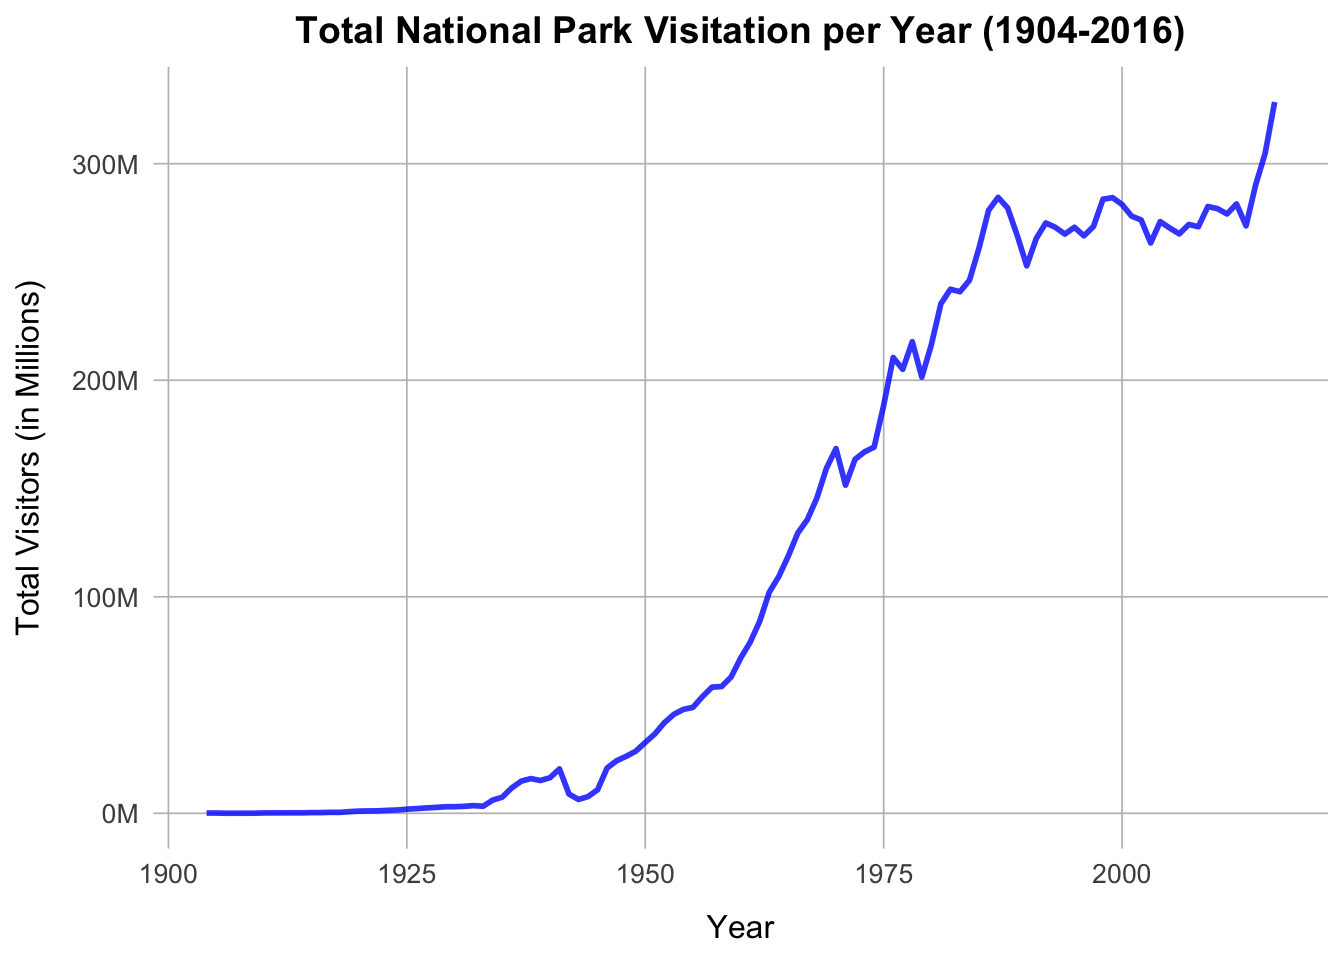
\includegraphics[width=400px]{NPS_Project_CharlesCoonce_files/figure-latex/Create a basic Line Plot of Total Visitation-1}

\begin{center}\rule{0.5\linewidth}{0.5pt}\end{center}

This plot shows how visitor numbers have changed over time. It appears
there is an overall increasing trend in the number of visitors, which
could be attributed to a variety of factors that would require a deeper
dive.

\begin{figure}
\centering
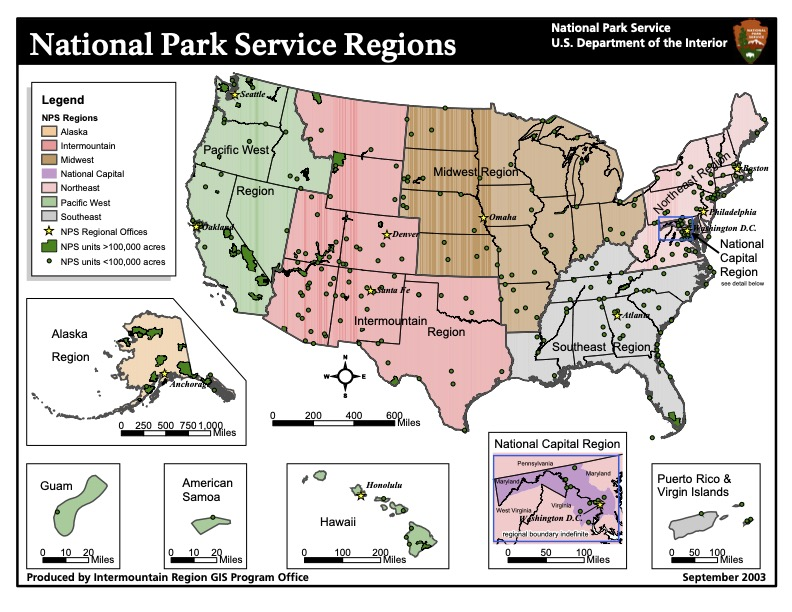
\includegraphics[width=5.20833in,height=6.25in]{assets/nps_regions_map.jpg}
\caption{National Parks Service Regions - This poster explains the
region categories used in this data set.}
\end{figure}

\newpage

\subsection{Regions}\label{regions}

The data set is subdivided into regions as shown in the info graphic
above.

I am only interested in regions near me. So I am going to look at the
region I am in as well as surrounding regions. I need to group and
filter my data set to get the appropriate observations.

\begin{Shaded}
\begin{Highlighting}[]
  \DocumentationTok{\#\# group and filter by region}
\NormalTok{region\_total }\OtherTok{\textless{}{-}}\NormalTok{ data\_clean }\SpecialCharTok{\%\textgreater{}\%}
  \FunctionTok{filter}\NormalTok{(Region }\SpecialCharTok{==} \StringTok{"PW"} \SpecialCharTok{|}\NormalTok{ Region }\SpecialCharTok{==} \StringTok{"IM"} \SpecialCharTok{|}
\NormalTok{         Region }\SpecialCharTok{==} \StringTok{"MW"}\NormalTok{) }\SpecialCharTok{\%\textgreater{}\%}
  \FunctionTok{group\_by}\NormalTok{(YearRaw, Region) }\SpecialCharTok{\%\textgreater{}\%} 
  \FunctionTok{summarise}\NormalTok{(}\AttributeTok{Total =} \FunctionTok{sum}\NormalTok{(Visitors), }\AttributeTok{.groups =} \StringTok{"rowwise"}\NormalTok{) }\SpecialCharTok{\%\textgreater{}\%}
  \FunctionTok{na.omit}\NormalTok{()}
\end{Highlighting}
\end{Shaded}

\begin{center}\rule{0.5\linewidth}{0.5pt}\end{center}

\includegraphics{NPS_Project_CharlesCoonce_files/figure-latex/Plot 2-1.pdf}

\begin{center}\rule{0.5\linewidth}{0.5pt}\end{center}

These plots show that Intermountain and Pacific West regions have seen
the steepest increases in visits. I will focus my attention on these two
regions.

\phantomsection\label{visitation_trends_states}
\subsection{States}\label{states}

In order to show total visitation by state I need to filter and group my
data set.

\begin{Shaded}
\begin{Highlighting}[]
  \DocumentationTok{\#\# Group by State}
\NormalTok{state\_data }\OtherTok{\textless{}{-}}\NormalTok{ data\_clean }\SpecialCharTok{\%\textgreater{}\%}
  \FunctionTok{group\_by}\NormalTok{(State) }\SpecialCharTok{\%\textgreater{}\%}
  \FunctionTok{summarise}\NormalTok{(}\AttributeTok{Total =} \FunctionTok{sum}\NormalTok{(Visitors)) }\SpecialCharTok{\%\textgreater{}\%}
  \FunctionTok{filter}\NormalTok{(State }\SpecialCharTok{\%in\%} \FunctionTok{c}\NormalTok{(}\StringTok{"WA"}\NormalTok{, }\StringTok{"OR"}\NormalTok{, }\StringTok{"CA"}\NormalTok{, }\StringTok{"MT"}\NormalTok{, }\StringTok{"WY"}\NormalTok{, }
                      \StringTok{"CO"}\NormalTok{, }\StringTok{"UT"}\NormalTok{, }\StringTok{"NV"}\NormalTok{, }\StringTok{"ND"}\NormalTok{, }\StringTok{"SD"}\NormalTok{, }
                      \StringTok{"NE"}\NormalTok{, }\StringTok{"ID"}\NormalTok{, }\StringTok{"AZ"}\NormalTok{, }\StringTok{"NM"}\NormalTok{))}
\end{Highlighting}
\end{Shaded}

Next, I need to add location data in order to create a heat map of my
new data. I can use the `usmap' package to create an interesting plot.

\begin{Shaded}
\begin{Highlighting}[]
  \DocumentationTok{\#\# Get the states map data from usmap}
\NormalTok{states\_map }\OtherTok{\textless{}{-}}\NormalTok{ usmap}\SpecialCharTok{::}\FunctionTok{us\_map}\NormalTok{(}\AttributeTok{regions =} \StringTok{"states"}\NormalTok{) }\SpecialCharTok{\%\textgreater{}\%}
  \FunctionTok{filter}\NormalTok{(abbr }\SpecialCharTok{\%in\%} \FunctionTok{c}\NormalTok{(}\StringTok{"WA"}\NormalTok{, }\StringTok{"OR"}\NormalTok{, }\StringTok{"CA"}\NormalTok{, }\StringTok{"MT"}\NormalTok{, }\StringTok{"WY"}\NormalTok{, }\StringTok{"CO"}\NormalTok{, }
                     \StringTok{"UT"}\NormalTok{, }\StringTok{"NV"}\NormalTok{, }\StringTok{"ND"}\NormalTok{, }\StringTok{"SD"}\NormalTok{, }\StringTok{"NE"}\NormalTok{, }\StringTok{"ID"}\NormalTok{, }
                     \StringTok{"AZ"}\NormalTok{, }\StringTok{"NM"}\NormalTok{))}

  \DocumentationTok{\#\# Merge visitor data with map data}
\NormalTok{merged\_data }\OtherTok{\textless{}{-}} \FunctionTok{merge}\NormalTok{(states\_map, state\_data, }\AttributeTok{by.x =} \StringTok{"abbr"}\NormalTok{, }
                     \AttributeTok{by.y =} \StringTok{"State"}\NormalTok{, }\AttributeTok{all.x =} \ConstantTok{TRUE}\NormalTok{)}
\end{Highlighting}
\end{Shaded}

Now I can prepare my base layer for adding multiple data visualizations.

\begin{Shaded}
\begin{Highlighting}[]
\NormalTok{p3 }\OtherTok{\textless{}{-}} \FunctionTok{ggplot}\NormalTok{() }\SpecialCharTok{+}
  \FunctionTok{geom\_sf}\NormalTok{(}\AttributeTok{data =}\NormalTok{ merged\_data, }\FunctionTok{aes}\NormalTok{(}\AttributeTok{fill =}\NormalTok{ Total), }\AttributeTok{color =} \StringTok{"black"}\NormalTok{) }\SpecialCharTok{+}
  \FunctionTok{scale\_fill\_continuous}\NormalTok{(}
    \AttributeTok{labels =}\NormalTok{ scales}\SpecialCharTok{::}\NormalTok{comma, }
    \AttributeTok{low =} \StringTok{"white"}\NormalTok{, }
    \AttributeTok{high =} \StringTok{"red"}\NormalTok{, }
    \AttributeTok{name =} \StringTok{"All Time Visits"}\NormalTok{, }
    \AttributeTok{na.value =} \StringTok{"gray"}
\NormalTok{  ) }\SpecialCharTok{+}
  \FunctionTok{theme\_void}\NormalTok{() }\SpecialCharTok{+}
  \FunctionTok{labs}\NormalTok{(}\AttributeTok{title =} \StringTok{"Heatmap of Total National Park Visits"}\NormalTok{,}
       \AttributeTok{subtitle =} \StringTok{"by Selected Western US States"}\NormalTok{) }\SpecialCharTok{+}
  \FunctionTok{theme}\NormalTok{(}
    \AttributeTok{legend.position =} \StringTok{"right"}\NormalTok{,}
    \AttributeTok{legend.title =} \FunctionTok{element\_text}\NormalTok{(}\AttributeTok{size =} \DecValTok{14}\NormalTok{, }\AttributeTok{face =} \StringTok{"bold"}\NormalTok{), }
    \AttributeTok{legend.text =} \FunctionTok{element\_text}\NormalTok{(}\AttributeTok{size =} \DecValTok{12}\NormalTok{), }
    \AttributeTok{legend.key.size =} \FunctionTok{unit}\NormalTok{(}\FloatTok{1.5}\NormalTok{, }\StringTok{"cm"}\NormalTok{),  }
    \AttributeTok{plot.title =} \FunctionTok{element\_text}\NormalTok{(}\AttributeTok{size =} \DecValTok{16}\NormalTok{, }\AttributeTok{face =} \StringTok{"bold"}\NormalTok{, }\AttributeTok{hjust =} \FloatTok{0.5}\NormalTok{),}
    \AttributeTok{plot.subtitle =} \FunctionTok{element\_text}\NormalTok{(}\AttributeTok{size =} \DecValTok{14}\NormalTok{, }\AttributeTok{hjust =} \FloatTok{0.5}\NormalTok{),}
\NormalTok{  )}

\FunctionTok{print}\NormalTok{(p3)}
\end{Highlighting}
\end{Shaded}

\includegraphics{NPS_Project_CharlesCoonce_files/figure-latex/Create Base Map for Map Plot-1.pdf}

\newpage

This heat map shows which states have the most visitors. Based on the
results, I will pick the top parks in California, Wyoming, and
Washington. I'd like to start thinking about weighing the distance from
my home and the number of visitors to see if it can help me decide.

\phantomsection\label{visitation_trends_parks}
I will need to find another data set to add latitude and longitude
values for the top parks. and add that information into my top parks
data I started preparing below.

\begin{Shaded}
\begin{Highlighting}[]
\NormalTok{top\_parks }\OtherTok{\textless{}{-}}\NormalTok{ data\_clean }\SpecialCharTok{\%\textgreater{}\%}
  \FunctionTok{group\_by}\NormalTok{(Unit.Name, State) }\SpecialCharTok{\%\textgreater{}\%}
  \FunctionTok{summarise}\NormalTok{(}\AttributeTok{Total =} \FunctionTok{sum}\NormalTok{(Visitors), }\AttributeTok{.groups =} \StringTok{"rowwise"}\NormalTok{) }\SpecialCharTok{\%\textgreater{}\%}
  \FunctionTok{arrange}\NormalTok{(}\FunctionTok{desc}\NormalTok{(Total)) }\SpecialCharTok{\%\textgreater{}\%}
  \FunctionTok{filter}\NormalTok{(State }\SpecialCharTok{\%in\%} \FunctionTok{c}\NormalTok{(}\StringTok{"WA"}\NormalTok{, }\StringTok{"OR"}\NormalTok{, }\StringTok{"CA"}\NormalTok{, }\StringTok{"MT"}\NormalTok{, }\StringTok{"WY"}\NormalTok{, }
                      \StringTok{"CO"}\NormalTok{, }\StringTok{"UT"}\NormalTok{, }\StringTok{"NV"}\NormalTok{, }\StringTok{"ND"}\NormalTok{, }\StringTok{"SD"}\NormalTok{, }
                      \StringTok{"NE"}\NormalTok{, }\StringTok{"ID"}\NormalTok{, }\StringTok{"AZ"}\NormalTok{, }\StringTok{"NM"}\NormalTok{))}
\end{Highlighting}
\end{Shaded}

I was able to compile the coordinates for a number of the most visited
parks. I need to create a data frame before I can merge my top parks
data with these locations.

\begin{Shaded}
\begin{Highlighting}[]
  \DocumentationTok{\#\# Creating a new data frame from the coordinates I compiled}
\NormalTok{geo\_data }\OtherTok{\textless{}{-}} \FunctionTok{read\_csv}\NormalTok{(}\StringTok{"\textasciitilde{}/Documents/GitHub/National\_Parks\_Project/assets/Data Sources/geo\_data\_processed.txt"}\NormalTok{, }\AttributeTok{col\_types =} \FunctionTok{cols}\NormalTok{(}\AttributeTok{Lat =} \FunctionTok{col\_number}\NormalTok{(),}
    \AttributeTok{Long =} \FunctionTok{col\_number}\NormalTok{()))}
\end{Highlighting}
\end{Shaded}

\begin{Shaded}
\begin{Highlighting}[]
 \DocumentationTok{\#\# adding coordinates to my list of top parks}
\NormalTok{top\_parks\_merged }\OtherTok{\textless{}{-}} \FunctionTok{merge}\NormalTok{(top\_parks, geo\_data, }
                     \AttributeTok{by.x =} \StringTok{"Unit.Name"}\NormalTok{, }\AttributeTok{by.y =} \StringTok{"Park Name"}\NormalTok{)}

  \DocumentationTok{\#\# rearranging columns to make manipulation easier}
\NormalTok{top\_parks\_rearranged }\OtherTok{\textless{}{-}} \FunctionTok{select}\NormalTok{(top\_parks\_merged, Unit.Name, State.x, Total, Longitude, Latitude)}
\end{Highlighting}
\end{Shaded}

After Merging, I now need to convert the Longitude and Latitude to the
`usmap' coordinate system in order to map locations onto my base layer.

\begin{Shaded}
\begin{Highlighting}[]
\NormalTok{states\_to\_include }\OtherTok{\textless{}{-}} \FunctionTok{c}\NormalTok{(}\StringTok{"WA"}\NormalTok{, }\StringTok{"OR"}\NormalTok{, }\StringTok{"CA"}\NormalTok{, }\StringTok{"MT"}\NormalTok{, }\StringTok{"WY"}\NormalTok{, }\StringTok{"CO"}\NormalTok{, }\StringTok{"UT"}\NormalTok{, }\StringTok{"NV"}\NormalTok{, }\StringTok{"ND"}\NormalTok{, }\StringTok{"SD"}\NormalTok{, }\StringTok{"NE"}\NormalTok{, }\StringTok{"ID"}\NormalTok{, }\StringTok{"AZ"}\NormalTok{, }\StringTok{"NM"}\NormalTok{)}

\NormalTok{states\_map }\OtherTok{\textless{}{-}}\NormalTok{ usmap}\SpecialCharTok{::}\FunctionTok{us\_map}\NormalTok{(}\AttributeTok{regions =} \StringTok{"states"}\NormalTok{) }\SpecialCharTok{\%\textgreater{}\%}
  \FunctionTok{filter}\NormalTok{(abbr }\SpecialCharTok{\%in\%}\NormalTok{ states\_to\_include)}

\NormalTok{top\_parks\_rearranged\_sf }\OtherTok{\textless{}{-}} \FunctionTok{st\_as\_sf}\NormalTok{(top\_parks\_rearranged, }
                                    \AttributeTok{coords =} \FunctionTok{c}\NormalTok{(}\StringTok{"Longitude"}\NormalTok{, }\StringTok{"Latitude"}\NormalTok{), }
                                    \AttributeTok{crs =} \DecValTok{4326}\NormalTok{)}
\end{Highlighting}
\end{Shaded}

Now I can create a plot to summarize my findings.

\begin{center}\rule{0.5\linewidth}{0.5pt}\end{center}

\begin{Shaded}
\begin{Highlighting}[]
\NormalTok{base\_map }\OtherTok{\textless{}{-}} \FunctionTok{ggplot}\NormalTok{() }\SpecialCharTok{+}
  \FunctionTok{geom\_sf}\NormalTok{(}\AttributeTok{data =}\NormalTok{ states\_map, }\AttributeTok{fill =} \StringTok{"white"}\NormalTok{, }\AttributeTok{color =} \StringTok{"black"}\NormalTok{ ) }\SpecialCharTok{+}
  \FunctionTok{theme\_minimal}\NormalTok{() }\SpecialCharTok{+}
  \FunctionTok{labs}\NormalTok{(}\AttributeTok{title =} \StringTok{"Western United States National Parks"}\NormalTok{,}
       \AttributeTok{subtitle =} \StringTok{"All Time Visitation"}\NormalTok{)}\SpecialCharTok{+}
  \FunctionTok{theme}\NormalTok{(}\AttributeTok{plot.title =} \FunctionTok{element\_text}\NormalTok{(}\AttributeTok{face =} \StringTok{"bold"}\NormalTok{, }\AttributeTok{size =} \DecValTok{18}\NormalTok{, }\AttributeTok{hjust =} \FloatTok{0.5}\NormalTok{),}
        \AttributeTok{plot.subtitle =} \FunctionTok{element\_text}\NormalTok{(}\AttributeTok{size =} \DecValTok{14}\NormalTok{, }\AttributeTok{hjust =} \FloatTok{0.5}\NormalTok{),}
        \AttributeTok{plot.caption =} \FunctionTok{element\_text}\NormalTok{(}\AttributeTok{size =} \DecValTok{10}\NormalTok{, }\AttributeTok{hjust =} \DecValTok{1}\NormalTok{),}
        \AttributeTok{panel.grid.major =} \FunctionTok{element\_blank}\NormalTok{(),}
        \AttributeTok{panel.grid.minor =} \FunctionTok{element\_blank}\NormalTok{())}


\NormalTok{bubble\_plot }\OtherTok{\textless{}{-}}\NormalTok{ base\_map }\SpecialCharTok{+}
  \FunctionTok{geom\_sf}\NormalTok{(}\AttributeTok{data =}\NormalTok{ top\_parks\_rearranged\_sf, }\FunctionTok{aes}\NormalTok{(}\AttributeTok{size =}\NormalTok{ Total), }\AttributeTok{fill =} \StringTok{"dodgerblue3"}\NormalTok{, }\AttributeTok{color =} \StringTok{"blue"}\NormalTok{, }\AttributeTok{alpha =} \FloatTok{0.6}\NormalTok{, }\AttributeTok{shape =} \DecValTok{21}\NormalTok{) }\SpecialCharTok{+} 
  \FunctionTok{scale\_size\_continuous}\NormalTok{(}\AttributeTok{name =} \StringTok{"Total Visitors"}\NormalTok{, }
                        \AttributeTok{labels =}\NormalTok{ scales}\SpecialCharTok{::}\FunctionTok{label\_number}\NormalTok{(}\AttributeTok{big.mark =} \StringTok{","}\NormalTok{),}
                        \AttributeTok{transform =} \StringTok{"sqrt"}\NormalTok{) }\SpecialCharTok{+}
  \FunctionTok{theme}\NormalTok{(}\AttributeTok{legend.position =} \StringTok{"right"}\NormalTok{,}
        \AttributeTok{legend.title =} \FunctionTok{element\_text}\NormalTok{(}\AttributeTok{face =} \StringTok{"bold"}\NormalTok{, }\AttributeTok{size =} \DecValTok{12}\NormalTok{),}
        \AttributeTok{legend.text =} \FunctionTok{element\_text}\NormalTok{(}\AttributeTok{size =} \DecValTok{10}\NormalTok{))}

\FunctionTok{print}\NormalTok{(bubble\_plot)}
\end{Highlighting}
\end{Shaded}

\includegraphics{NPS_Project_CharlesCoonce_files/figure-latex/bubble Plot-1.pdf}

\begin{center}\rule{0.5\linewidth}{0.5pt}\end{center}

Now that I have a better idea of where specific top parks are I can
start narrowing my search. I think I should consider distance from my
home.

\phantomsection\label{distance_analysis}
\subsection{Distance Analysis}\label{distance-analysis}

I will start by loading and converting my hometown coordinates to the
`usmap' coordinate system.

\begin{Shaded}
\begin{Highlighting}[]
  \DocumentationTok{\#\# Coordinates for Helena, Montana}
\NormalTok{helena\_coords }\OtherTok{\textless{}{-}} \FunctionTok{data.frame}\NormalTok{(}\AttributeTok{Latitude =} \FloatTok{46.5891}\NormalTok{, }\AttributeTok{Longitude =} \SpecialCharTok{{-}}\FloatTok{112.0372}\NormalTok{)}

\NormalTok{helena\_coords\_transformed\_sf }\OtherTok{\textless{}{-}} \FunctionTok{st\_as\_sf}\NormalTok{(helena\_coords, }
                                    \AttributeTok{coords =} \FunctionTok{c}\NormalTok{(}\StringTok{"Longitude"}\NormalTok{, }\StringTok{"Latitude"}\NormalTok{), }
                                    \AttributeTok{crs =} \DecValTok{4326}\NormalTok{)}

\NormalTok{top\_parks\_merged\_sf }\OtherTok{\textless{}{-}} \FunctionTok{st\_as\_sf}\NormalTok{(top\_parks\_merged, }
                                    \AttributeTok{coords =} \FunctionTok{c}\NormalTok{(}\StringTok{"Longitude"}\NormalTok{, }\StringTok{"Latitude"}\NormalTok{), }
                                    \AttributeTok{crs =} \DecValTok{4326}\NormalTok{)}
\end{Highlighting}
\end{Shaded}

\begin{Shaded}
\begin{Highlighting}[]
  \DocumentationTok{\#\# Function for getting route coordinates for each park}
\NormalTok{get\_route }\OtherTok{\textless{}{-}} \ControlFlowTok{function}\NormalTok{(start, end) \{}
\NormalTok{  url }\OtherTok{\textless{}{-}} \FunctionTok{paste0}\NormalTok{(}
    \StringTok{"http://router.project{-}osrm.org/route/v1/driving/"}\NormalTok{,}
\NormalTok{    start[}\StringTok{"lon"}\NormalTok{], }\StringTok{","}\NormalTok{, start[}\StringTok{"lat"}\NormalTok{], }\StringTok{";"}\NormalTok{,}
\NormalTok{    end[}\StringTok{"Longitude"}\NormalTok{], }\StringTok{","}\NormalTok{, end[}\StringTok{"Latitude"}\NormalTok{],}
    \StringTok{"?overview=full\&geometries=geojson"}
\NormalTok{  )}
  
\NormalTok{  response }\OtherTok{\textless{}{-}}\NormalTok{ httr}\SpecialCharTok{::}\FunctionTok{GET}\NormalTok{(url)}
\NormalTok{  route }\OtherTok{\textless{}{-}}\NormalTok{ jsonlite}\SpecialCharTok{::}\FunctionTok{fromJSON}\NormalTok{(}\FunctionTok{content}\NormalTok{(response, }\StringTok{"text"}\NormalTok{, }\AttributeTok{encoding =} \StringTok{"UTF{-}8"}\NormalTok{))}
\NormalTok{  route\_coords }\OtherTok{\textless{}{-}}\NormalTok{ route}\SpecialCharTok{$}\NormalTok{routes}\SpecialCharTok{$}\NormalTok{geometry}\SpecialCharTok{$}\NormalTok{coordinates[[}\DecValTok{1}\NormalTok{]]}
\NormalTok{  route\_coords\_df }\OtherTok{\textless{}{-}} \FunctionTok{data.frame}\NormalTok{(}
    \AttributeTok{lon =}\NormalTok{ route\_coords[, }\DecValTok{1}\NormalTok{],}
    \AttributeTok{lat =}\NormalTok{ route\_coords[, }\DecValTok{2}\NormalTok{]}
\NormalTok{  )}
  \FunctionTok{return}\NormalTok{(route\_coords\_df)}
\NormalTok{\}}

  \DocumentationTok{\#\# Helena (Start Location) coordinates}
\NormalTok{start }\OtherTok{\textless{}{-}} \FunctionTok{c}\NormalTok{(}\AttributeTok{lat =} \FloatTok{46.5891}\NormalTok{, }\AttributeTok{lon =} \SpecialCharTok{{-}}\FloatTok{112.0372}\NormalTok{)}

\NormalTok{routes\_list }\OtherTok{\textless{}{-}} \FunctionTok{lapply}\NormalTok{(}\DecValTok{1}\SpecialCharTok{:}\FunctionTok{nrow}\NormalTok{(top\_parks\_merged), }\ControlFlowTok{function}\NormalTok{(i) \{}
\NormalTok{  end }\OtherTok{\textless{}{-}}\NormalTok{ top\_parks\_merged[i, ]}
\NormalTok{  route\_df }\OtherTok{\textless{}{-}} \FunctionTok{get\_route}\NormalTok{(start, end)}
\NormalTok{  route\_df}\SpecialCharTok{$}\NormalTok{park }\OtherTok{\textless{}{-}}\NormalTok{ top\_parks\_merged}\SpecialCharTok{$}\NormalTok{Unit.Name[i]}
  \FunctionTok{return}\NormalTok{(route\_df)}
\NormalTok{\})}

\NormalTok{all\_routes }\OtherTok{\textless{}{-}} \FunctionTok{do.call}\NormalTok{(rbind, routes\_list)}
\end{Highlighting}
\end{Shaded}

\begin{Shaded}
\begin{Highlighting}[]
\CommentTok{\# Conversion factor from meters to miles}
\NormalTok{meters\_to\_miles }\OtherTok{\textless{}{-}} \FloatTok{1609.34}

\CommentTok{\# Function to calculate total distance of a route in miles}
\NormalTok{calculate\_total\_distance\_miles }\OtherTok{\textless{}{-}} \ControlFlowTok{function}\NormalTok{(df) \{}
  \CommentTok{\# Ensure that lon and lat columns are numeric}
\NormalTok{  df}\SpecialCharTok{$}\NormalTok{lon }\OtherTok{\textless{}{-}} \FunctionTok{as.numeric}\NormalTok{(df}\SpecialCharTok{$}\NormalTok{lon)}
\NormalTok{  df}\SpecialCharTok{$}\NormalTok{lat }\OtherTok{\textless{}{-}} \FunctionTok{as.numeric}\NormalTok{(df}\SpecialCharTok{$}\NormalTok{lat)}
  
  \CommentTok{\# Compute distances between consecutive points}
\NormalTok{  coords }\OtherTok{\textless{}{-}} \FunctionTok{as.matrix}\NormalTok{(df[, }\FunctionTok{c}\NormalTok{(}\StringTok{"lon"}\NormalTok{, }\StringTok{"lat"}\NormalTok{)])}
\NormalTok{  distances }\OtherTok{\textless{}{-}} \FunctionTok{distVincentySphere}\NormalTok{(coords[}\DecValTok{1}\SpecialCharTok{:}\NormalTok{(}\FunctionTok{nrow}\NormalTok{(coords) }\SpecialCharTok{{-}} \DecValTok{1}\NormalTok{), ], coords[}\DecValTok{2}\SpecialCharTok{:}\FunctionTok{nrow}\NormalTok{(coords), ])}
  
  \CommentTok{\# Sum distances and convert to miles}
\NormalTok{  total\_distance\_meters }\OtherTok{\textless{}{-}} \FunctionTok{sum}\NormalTok{(distances)}
\NormalTok{  total\_distance\_miles }\OtherTok{\textless{}{-}}\NormalTok{ total\_distance\_meters }\SpecialCharTok{/}\NormalTok{ meters\_to\_miles}
  \FunctionTok{return}\NormalTok{(total\_distance\_miles)}
\NormalTok{\}}

\CommentTok{\# Apply the function to each data frame in routes\_list}
\NormalTok{total\_distances\_miles }\OtherTok{\textless{}{-}} \FunctionTok{sapply}\NormalTok{(routes\_list, calculate\_total\_distance\_miles)}

\CommentTok{\# Add total distances (in miles) to each data frame in routes\_list}
\NormalTok{routes\_list\_with\_distance\_miles }\OtherTok{\textless{}{-}} \FunctionTok{Map}\NormalTok{(}\ControlFlowTok{function}\NormalTok{(df, dist) \{}
\NormalTok{  df}\SpecialCharTok{$}\NormalTok{total\_distance\_miles }\OtherTok{\textless{}{-}}\NormalTok{ dist}
  \FunctionTok{return}\NormalTok{(df)}
\NormalTok{\}, routes\_list, total\_distances\_miles)}

\NormalTok{all\_routes }\OtherTok{\textless{}{-}} \FunctionTok{bind\_rows}\NormalTok{(routes\_list\_with\_distance\_miles)}
\end{Highlighting}
\end{Shaded}

\begin{Shaded}
\begin{Highlighting}[]
\NormalTok{route\_sf }\OtherTok{\textless{}{-}} \FunctionTok{st\_as\_sf}\NormalTok{(all\_routes, }\AttributeTok{coords =} \FunctionTok{c}\NormalTok{(}\StringTok{"lon"}\NormalTok{, }\StringTok{"lat"}\NormalTok{), }\AttributeTok{crs =} \DecValTok{4326}\NormalTok{)}

\CommentTok{\# Add a column for distance categories for better visualization}
\NormalTok{all\_routes}\SpecialCharTok{$}\NormalTok{distance\_category }\OtherTok{\textless{}{-}} \FunctionTok{cut}\NormalTok{(}
\NormalTok{  all\_routes}\SpecialCharTok{$}\NormalTok{total\_distance\_miles,}
  \AttributeTok{breaks =} \FunctionTok{c}\NormalTok{(}\DecValTok{0}\NormalTok{, }\DecValTok{10}\NormalTok{, }\DecValTok{50}\NormalTok{, }\DecValTok{100}\NormalTok{, }\DecValTok{200}\NormalTok{, }\ConstantTok{Inf}\NormalTok{), }
  \AttributeTok{labels =} \FunctionTok{c}\NormalTok{(}\StringTok{"0{-}10 miles"}\NormalTok{, }\StringTok{"10{-}50 miles"}\NormalTok{, }\StringTok{"50{-}100 miles"}\NormalTok{, }\StringTok{"100{-}200 miles"}\NormalTok{, }\StringTok{"200+ miles"}\NormalTok{)}
\NormalTok{)}

\NormalTok{p }\OtherTok{\textless{}{-}}\NormalTok{ base\_map }\SpecialCharTok{+}
  \FunctionTok{geom\_sf}\NormalTok{(}\AttributeTok{data =}\NormalTok{ route\_sf, }\FunctionTok{aes}\NormalTok{(}\AttributeTok{color =}\NormalTok{ total\_distance\_miles), }\AttributeTok{size =} \FloatTok{0.1}\NormalTok{) }\SpecialCharTok{+}
  \FunctionTok{labs}\NormalTok{(}\AttributeTok{title =} \StringTok{"Routes from Helena, MT to National Parks"}\NormalTok{,}
       \AttributeTok{subtitle =} \StringTok{"Distances visualized with a color gradient"}\NormalTok{,}
       \AttributeTok{x =} \StringTok{"Longitude"}\NormalTok{, }\AttributeTok{y =} \StringTok{"Latitude"}\NormalTok{,}
       \AttributeTok{color =} \StringTok{"Distance (miles)"}\NormalTok{) }\SpecialCharTok{+}
  \FunctionTok{theme\_minimal}\NormalTok{() }\SpecialCharTok{+}
  \FunctionTok{theme}\NormalTok{(}
    \AttributeTok{plot.title =} \FunctionTok{element\_text}\NormalTok{(}\AttributeTok{face =} \StringTok{"bold"}\NormalTok{, }\AttributeTok{size =} \DecValTok{16}\NormalTok{, }\AttributeTok{hjust =} \FloatTok{0.5}\NormalTok{, }\AttributeTok{vjust =} \FloatTok{0.5}\NormalTok{),}
    \AttributeTok{plot.subtitle =} \FunctionTok{element\_text}\NormalTok{(}\AttributeTok{size =} \DecValTok{12}\NormalTok{, }\AttributeTok{hjust =} \FloatTok{0.5}\NormalTok{),}
    \AttributeTok{legend.title =} \FunctionTok{element\_text}\NormalTok{(}\AttributeTok{size =} \DecValTok{12}\NormalTok{),}
    \AttributeTok{legend.text =} \FunctionTok{element\_text}\NormalTok{(}\AttributeTok{size =} \DecValTok{10}\NormalTok{)}
\NormalTok{  ) }\SpecialCharTok{+}
  \FunctionTok{scale\_color\_viridis\_c}\NormalTok{()}

\FunctionTok{print}\NormalTok{(p)}
\end{Highlighting}
\end{Shaded}

\includegraphics{NPS_Project_CharlesCoonce_files/figure-latex/plot routes-1.pdf}

\begin{center}\rule{0.5\linewidth}{0.5pt}\end{center}

\phantomsection\label{cluster_parks}
\section{Re-Defining the problem}\label{re-defining-the-problem}

After seeing this visualization, I want to pivot to a new problem. How I
can optimize seeing multiple parks per trip rather than trying to choose
one park. There are too many nearby! I need to use a clustering model to
group the parks by looking at their distances from each other. To do
this I need to use a hierarchical cluster function.

\begin{Shaded}
\begin{Highlighting}[]
  \DocumentationTok{\#\# Perform a hierarchical clustering}

\NormalTok{top\_parks\_cluster }\OtherTok{\textless{}{-}}\NormalTok{ top\_parks\_merged}

\CommentTok{\# Function to calculate approximate distance between two points}
\NormalTok{calculate\_distance }\OtherTok{\textless{}{-}} \ControlFlowTok{function}\NormalTok{(lat1, lon1, lat2, lon2) \{}
  \FunctionTok{distVincentySphere}\NormalTok{(}\FunctionTok{c}\NormalTok{(lon1, lat1), }\FunctionTok{c}\NormalTok{(lon2, lat2)) }\SpecialCharTok{/} \DecValTok{1000}  \CommentTok{\# Convert meters to kilometers}
\NormalTok{\}}

\CommentTok{\# Create a distance matrix}
\NormalTok{num\_parks }\OtherTok{\textless{}{-}} \FunctionTok{nrow}\NormalTok{(top\_parks\_merged)}
\NormalTok{distance\_matrix }\OtherTok{\textless{}{-}} \FunctionTok{matrix}\NormalTok{(}\DecValTok{0}\NormalTok{, }\AttributeTok{nrow =}\NormalTok{ num\_parks, }\AttributeTok{ncol =}\NormalTok{ num\_parks, }\AttributeTok{dimnames =} \FunctionTok{list}\NormalTok{(top\_parks\_cluster}\SpecialCharTok{$}\NormalTok{name, top\_parks\_cluster}\SpecialCharTok{$}\NormalTok{name))}

\ControlFlowTok{for}\NormalTok{ (i }\ControlFlowTok{in} \DecValTok{1}\SpecialCharTok{:}\NormalTok{num\_parks) \{}
  \ControlFlowTok{for}\NormalTok{ (j }\ControlFlowTok{in} \DecValTok{1}\SpecialCharTok{:}\NormalTok{num\_parks) \{}
    \ControlFlowTok{if}\NormalTok{ (i }\SpecialCharTok{!=}\NormalTok{ j) \{}
\NormalTok{      lat1 }\OtherTok{\textless{}{-}}\NormalTok{ top\_parks\_cluster}\SpecialCharTok{$}\NormalTok{Latitude[i]}
\NormalTok{      lon1 }\OtherTok{\textless{}{-}}\NormalTok{ top\_parks\_cluster}\SpecialCharTok{$}\NormalTok{Longitude[i]}
\NormalTok{      lat2 }\OtherTok{\textless{}{-}}\NormalTok{ top\_parks\_cluster}\SpecialCharTok{$}\NormalTok{Latitude[j]}
\NormalTok{      lon2 }\OtherTok{\textless{}{-}}\NormalTok{ top\_parks\_cluster}\SpecialCharTok{$}\NormalTok{Longitude[j]}
\NormalTok{      distance }\OtherTok{\textless{}{-}} \FunctionTok{calculate\_distance}\NormalTok{(lat1, lon1, lat2, lon2)}
\NormalTok{      distance\_matrix[i, j] }\OtherTok{\textless{}{-}}\NormalTok{ distance}
\NormalTok{    \}}
\NormalTok{  \}}
\NormalTok{\}}

\CommentTok{\# Convert the distance matrix to a data frame}
\NormalTok{distance\_df }\OtherTok{\textless{}{-}} \FunctionTok{as.data.frame}\NormalTok{(}\FunctionTok{as.table}\NormalTok{(distance\_matrix))}
\FunctionTok{names}\NormalTok{(distance\_df) }\OtherTok{\textless{}{-}} \FunctionTok{c}\NormalTok{(}\StringTok{"from"}\NormalTok{, }\StringTok{"to"}\NormalTok{, }\StringTok{"distance\_km"}\NormalTok{)}
  
  \DocumentationTok{\#\# Creating distance matrix}
\NormalTok{dist\_matrix }\OtherTok{\textless{}{-}} \FunctionTok{dist}\NormalTok{(top\_parks\_cluster[,}\FunctionTok{c}\NormalTok{(}\StringTok{\textquotesingle{}Longitude\textquotesingle{}}\NormalTok{, }\StringTok{\textquotesingle{}Latitude\textquotesingle{}}\NormalTok{)])}
\NormalTok{clusters }\OtherTok{\textless{}{-}} \FunctionTok{hclust}\NormalTok{(dist\_matrix)}

  \DocumentationTok{\#\# Split into clusters of parks}
\NormalTok{park\_clusters }\OtherTok{\textless{}{-}} \FunctionTok{cutree}\NormalTok{(clusters, }\AttributeTok{k =} \DecValTok{5}\NormalTok{)}
\NormalTok{top\_parks\_cluster}\SpecialCharTok{$}\NormalTok{cluster }\OtherTok{\textless{}{-}}\NormalTok{ park\_clusters}
\end{Highlighting}
\end{Shaded}

\newpage

With my new set of clustered parks, I want to see how the clusters
worked out.

\begin{center}\rule{0.5\linewidth}{0.5pt}\end{center}

\includegraphics{NPS_Project_CharlesCoonce_files/figure-latex/Plot 7-1.pdf}

\begin{center}\rule{0.5\linewidth}{0.5pt}\end{center}

\phantomsection\label{cluster_parks_tsp}
Now I want to know what the most efficient way to drive from park to
park is so I will use the Traveling Salesman Problem (TSP). The TSP
finds shortest possible route that visits each city exactly once and
returns to the original city.

\begin{Shaded}
\begin{Highlighting}[]
  \DocumentationTok{\#\# Initialize an empty list to store results}
\NormalTok{tsp\_results }\OtherTok{\textless{}{-}} \FunctionTok{list}\NormalTok{()}

  \DocumentationTok{\#\# Loop through each cluster}
\ControlFlowTok{for}\NormalTok{ (i }\ControlFlowTok{in} \DecValTok{1}\SpecialCharTok{:}\FunctionTok{max}\NormalTok{(top\_parks\_cluster}\SpecialCharTok{$}\NormalTok{cluster)) \{}
    \DocumentationTok{\#\# Subset parks for the current cluster}
\NormalTok{  cluster\_parks }\OtherTok{\textless{}{-}}\NormalTok{ top\_parks\_cluster[top\_parks\_cluster}\SpecialCharTok{$}\NormalTok{cluster }\SpecialCharTok{==}\NormalTok{ i, ]}
  
    \DocumentationTok{\#\# Calculate the distance matrix for the current cluster}
\NormalTok{  dist\_matrix }\OtherTok{\textless{}{-}} \FunctionTok{as.dist}\NormalTok{(}\FunctionTok{distm}\NormalTok{(cluster\_parks[, }\FunctionTok{c}\NormalTok{(}\StringTok{"Longitude"}\NormalTok{, }\StringTok{"Latitude"}\NormalTok{)], }
\NormalTok{                               cluster\_parks[, }\FunctionTok{c}\NormalTok{(}\StringTok{"Longitude"}\NormalTok{, }\StringTok{"Latitude"}\NormalTok{)], }
                               \AttributeTok{fun =}\NormalTok{ distHaversine))}
  
    \DocumentationTok{\#\# Solve the TSP problem using the nearest neighbor heuristic}
\NormalTok{  tsp\_solution }\OtherTok{\textless{}{-}} \FunctionTok{solve\_TSP}\NormalTok{(}\FunctionTok{TSP}\NormalTok{(dist\_matrix), }\AttributeTok{method =} \StringTok{"nearest\_insertion"}\NormalTok{)}
  
    \DocumentationTok{\#\# Solution List}
\NormalTok{  tsp\_results[[}\FunctionTok{paste}\NormalTok{(}\StringTok{"Cluster"}\NormalTok{, i)]] }\OtherTok{\textless{}{-}}\NormalTok{ tsp\_solution}
\NormalTok{\}}
\end{Highlighting}
\end{Shaded}

Now that I have the results, I can visualize what the optimal route is.
In order to do that, I want to plot them all on the same map which will
require creating a function to compile all the data points into one
table.

\begin{Shaded}
\begin{Highlighting}[]
  \DocumentationTok{\#\# Function to create segments from the TSP solution}
\NormalTok{get\_tsp\_segments }\OtherTok{\textless{}{-}} \ControlFlowTok{function}\NormalTok{(cluster\_number, top\_parks\_cluster, tsp\_results) \{}
  
  \DocumentationTok{\#\# Filter the parks by the selected cluster}
\NormalTok{  selected\_cluster }\OtherTok{\textless{}{-}} \FunctionTok{filter}\NormalTok{(top\_parks\_cluster, cluster }\SpecialCharTok{==}\NormalTok{ cluster\_number)}
  
  \DocumentationTok{\#\# Retrieve the TSP order for the cluster}
\NormalTok{  tsp\_order }\OtherTok{\textless{}{-}}\NormalTok{ tsp\_results[[}\FunctionTok{paste}\NormalTok{(}\StringTok{"Cluster"}\NormalTok{, cluster\_number)]]}
  \FunctionTok{print}\NormalTok{(tsp\_order)}
\NormalTok{  tsp\_solution\_order }\OtherTok{\textless{}{-}} \FunctionTok{TOUR}\NormalTok{(tsp\_order)}
  
  \DocumentationTok{\#\# Order the parks according to the TSP solution}
\NormalTok{  ordered\_cluster }\OtherTok{\textless{}{-}}\NormalTok{ selected\_cluster[tsp\_solution\_order, ]}
  
  \DocumentationTok{\#\# Close the loop by returning to the starting point}
\NormalTok{  ordered\_cluster }\OtherTok{\textless{}{-}} \FunctionTok{rbind}\NormalTok{(ordered\_cluster, ordered\_cluster[}\DecValTok{1}\NormalTok{, ])}
  
  \DocumentationTok{\#\# Create segments for each leg of the TSP path}
\NormalTok{  segments }\OtherTok{\textless{}{-}} \FunctionTok{data.frame}\NormalTok{(}\AttributeTok{cluster =}\NormalTok{ cluster\_number,}
                         \AttributeTok{x =}\NormalTok{ ordered\_cluster}\SpecialCharTok{$}\NormalTok{Longitude[}\SpecialCharTok{{-}}\FunctionTok{nrow}\NormalTok{(ordered\_cluster)], }
                         \AttributeTok{y =}\NormalTok{ ordered\_cluster}\SpecialCharTok{$}\NormalTok{Latitude[}\SpecialCharTok{{-}}\FunctionTok{nrow}\NormalTok{(ordered\_cluster)], }
                         \AttributeTok{xend =}\NormalTok{ ordered\_cluster}\SpecialCharTok{$}\NormalTok{Longitude[}\SpecialCharTok{{-}}\DecValTok{1}\NormalTok{], }
                         \AttributeTok{yend =}\NormalTok{ ordered\_cluster}\SpecialCharTok{$}\NormalTok{Latitude[}\SpecialCharTok{{-}}\DecValTok{1}\NormalTok{]}
\NormalTok{                         )}
  
  \FunctionTok{return}\NormalTok{(segments)}
\NormalTok{\}}

  \DocumentationTok{\#\# Call the function}
\NormalTok{all\_segments }\OtherTok{\textless{}{-}} \FunctionTok{lapply}\NormalTok{(}\DecValTok{1}\SpecialCharTok{:}\FunctionTok{max}\NormalTok{(top\_parks\_cluster}\SpecialCharTok{$}\NormalTok{cluster), }\ControlFlowTok{function}\NormalTok{(cluster\_num) \{}
  \FunctionTok{get\_tsp\_segments}\NormalTok{(cluster\_num, top\_parks\_cluster, tsp\_results)}
\NormalTok{\})}
\end{Highlighting}
\end{Shaded}

\begin{verbatim}
## object of class 'TOUR' 
## result of method 'nearest_insertion' for 40 cities
## tour length: 5559751 
## object of class 'TOUR' 
## result of method 'nearest_insertion' for 15 cities
## tour length: 2831039 
## object of class 'TOUR' 
## result of method 'nearest_insertion' for 7 cities
## tour length: 2055642 
## object of class 'TOUR' 
## result of method 'nearest_insertion' for 22 cities
## tour length: 3481065 
## object of class 'TOUR' 
## result of method 'nearest_insertion' for 10 cities
## tour length: 1645687
\end{verbatim}

\begin{Shaded}
\begin{Highlighting}[]
\DocumentationTok{\#\# Combine all segments into one data frame}
\NormalTok{all\_segments\_df }\OtherTok{\textless{}{-}} \FunctionTok{do.call}\NormalTok{(rbind, all\_segments)}
\end{Highlighting}
\end{Shaded}

\begin{Shaded}
\begin{Highlighting}[]
\CommentTok{\# Function to get route coordinates from OSRM}
\NormalTok{get\_route\_osrm }\OtherTok{\textless{}{-}} \ControlFlowTok{function}\NormalTok{(start\_lon, start\_lat, end\_lon, end\_lat) \{}
\NormalTok{  url }\OtherTok{\textless{}{-}} \FunctionTok{paste0}\NormalTok{(}
    \StringTok{"http://router.project{-}osrm.org/route/v1/driving/"}\NormalTok{,}
\NormalTok{    start\_lon, }\StringTok{","}\NormalTok{, start\_lat, }\StringTok{";"}\NormalTok{, }
\NormalTok{    end\_lon, }\StringTok{","}\NormalTok{, end\_lat, }
    \StringTok{"?overview=full\&geometries=geojson"}
\NormalTok{  )}
  
\NormalTok{  response }\OtherTok{\textless{}{-}} \FunctionTok{GET}\NormalTok{(url)}
\NormalTok{  route }\OtherTok{\textless{}{-}} \FunctionTok{fromJSON}\NormalTok{(}\FunctionTok{content}\NormalTok{(response, }\StringTok{"text"}\NormalTok{, }\AttributeTok{encoding =} \StringTok{"UTF{-}8"}\NormalTok{))}
  
\NormalTok{  route\_coords }\OtherTok{\textless{}{-}}\NormalTok{ route}\SpecialCharTok{$}\NormalTok{routes}\SpecialCharTok{$}\NormalTok{geometry}\SpecialCharTok{$}\NormalTok{coordinates[[}\DecValTok{1}\NormalTok{]]}
\NormalTok{  route\_coords\_df }\OtherTok{\textless{}{-}} \FunctionTok{data.frame}\NormalTok{(}
    \AttributeTok{lon =}\NormalTok{ route\_coords[, }\DecValTok{1}\NormalTok{],}
    \AttributeTok{lat =}\NormalTok{ route\_coords[, }\DecValTok{2}\NormalTok{]}
\NormalTok{  )}
  \FunctionTok{return}\NormalTok{(route\_coords\_df)}
\NormalTok{\}}

\CommentTok{\# Apply the function to each row in the data frame}
\NormalTok{routes\_list\_cluster }\OtherTok{\textless{}{-}} \FunctionTok{lapply}\NormalTok{(}\DecValTok{1}\SpecialCharTok{:}\FunctionTok{nrow}\NormalTok{(all\_segments\_df), }\ControlFlowTok{function}\NormalTok{(i) \{}
\NormalTok{  start\_lon }\OtherTok{\textless{}{-}}\NormalTok{ all\_segments\_df}\SpecialCharTok{$}\NormalTok{x[i]}
\NormalTok{  start\_lat }\OtherTok{\textless{}{-}}\NormalTok{ all\_segments\_df}\SpecialCharTok{$}\NormalTok{y[i]}
\NormalTok{  end\_lon }\OtherTok{\textless{}{-}}\NormalTok{ all\_segments\_df}\SpecialCharTok{$}\NormalTok{xend[i]}
\NormalTok{  end\_lat }\OtherTok{\textless{}{-}}\NormalTok{ all\_segments\_df}\SpecialCharTok{$}\NormalTok{yend[i]}
  
\NormalTok{  route }\OtherTok{\textless{}{-}} \FunctionTok{get\_route\_osrm}\NormalTok{(start\_lon, start\_lat, end\_lon, end\_lat)}
  
\NormalTok{  route\_df }\OtherTok{\textless{}{-}} \FunctionTok{data.frame}\NormalTok{(}\AttributeTok{id =}\NormalTok{ i, }\AttributeTok{cluster =}\NormalTok{all\_segments\_df}\SpecialCharTok{$}\NormalTok{cluster[i], route)}
  
  \FunctionTok{return}\NormalTok{(route\_df)}
\NormalTok{\})}

\CommentTok{\# Combine all route data frames into one}
\NormalTok{all\_cluster\_routes\_df }\OtherTok{\textless{}{-}} \FunctionTok{do.call}\NormalTok{(rbind, routes\_list\_cluster)}

\CommentTok{\# Create an sf object from the combined data frame}
\NormalTok{routes\_sf }\OtherTok{\textless{}{-}} \FunctionTok{st\_as\_sf}\NormalTok{(all\_cluster\_routes\_df, }\AttributeTok{coords =} \FunctionTok{c}\NormalTok{(}\StringTok{"lon"}\NormalTok{, }\StringTok{"lat"}\NormalTok{), }\AttributeTok{crs =} \DecValTok{4326}\NormalTok{, }\AttributeTok{agr =} \StringTok{"constant"}\NormalTok{)}

\NormalTok{routes\_sf\_lines }\OtherTok{\textless{}{-}}\NormalTok{ routes\_sf }\SpecialCharTok{\%\textgreater{}\%}
  \FunctionTok{group\_by}\NormalTok{(id, cluster) }\SpecialCharTok{\%\textgreater{}\%}
  \FunctionTok{summarize}\NormalTok{(}\AttributeTok{geometry =} \FunctionTok{st\_combine}\NormalTok{(geometry)) }\SpecialCharTok{\%\textgreater{}\%}
  \FunctionTok{st\_cast}\NormalTok{(}\StringTok{"LINESTRING"}\NormalTok{)}
\end{Highlighting}
\end{Shaded}

\begin{verbatim}
## `summarise()` has grouped output by 'id'. You can override using the `.groups`
## argument.
\end{verbatim}

\newpage

\begin{center}\rule{0.5\linewidth}{0.5pt}\end{center}

\includegraphics{NPS_Project_CharlesCoonce_files/figure-latex/Plot 8-1.pdf}

\begin{center}\rule{0.5\linewidth}{0.5pt}\end{center}

\phantomsection\label{subcluster_parks}
\begin{Shaded}
\begin{Highlighting}[]
\CommentTok{\# Function to calculate approximate distance between two points}
\NormalTok{calculate\_distance }\OtherTok{\textless{}{-}} \ControlFlowTok{function}\NormalTok{(lat1, lon1, lat2, lon2) \{}
  \FunctionTok{distVincentySphere}\NormalTok{(}\FunctionTok{c}\NormalTok{(lon1, lat1), }\FunctionTok{c}\NormalTok{(lon2, lat2)) }\SpecialCharTok{/} \DecValTok{1000}  \CommentTok{\# Convert meters to kilometers}
\NormalTok{\}}

\NormalTok{perform\_hierarchical\_clustering }\OtherTok{\textless{}{-}} \ControlFlowTok{function}\NormalTok{(df) \{}
\NormalTok{  num\_parks }\OtherTok{\textless{}{-}} \FunctionTok{nrow}\NormalTok{(df)}

  \CommentTok{\# Create an empty distance matrix}
\NormalTok{  distance\_matrix }\OtherTok{\textless{}{-}} \FunctionTok{matrix}\NormalTok{(}\DecValTok{0}\NormalTok{, }\AttributeTok{nrow =}\NormalTok{ num\_parks, }\AttributeTok{ncol =}\NormalTok{ num\_parks, }
                            \AttributeTok{dimnames =} \FunctionTok{list}\NormalTok{(}\DecValTok{1}\SpecialCharTok{:}\NormalTok{num\_parks, }\DecValTok{1}\SpecialCharTok{:}\NormalTok{num\_parks))}
  
  \CommentTok{\# Populate the distance matrix}
  \ControlFlowTok{for}\NormalTok{ (i }\ControlFlowTok{in} \DecValTok{1}\SpecialCharTok{:}\NormalTok{num\_parks) \{}
    \ControlFlowTok{for}\NormalTok{ (j }\ControlFlowTok{in} \DecValTok{1}\SpecialCharTok{:}\NormalTok{num\_parks) \{}
      \ControlFlowTok{if}\NormalTok{ (i }\SpecialCharTok{!=}\NormalTok{ j) \{}
\NormalTok{        lat1 }\OtherTok{\textless{}{-}}\NormalTok{ df}\SpecialCharTok{$}\NormalTok{Latitude[i]}
\NormalTok{        lon1 }\OtherTok{\textless{}{-}}\NormalTok{ df}\SpecialCharTok{$}\NormalTok{Longitude[i]}
\NormalTok{        lat2 }\OtherTok{\textless{}{-}}\NormalTok{ df}\SpecialCharTok{$}\NormalTok{Latitude[j]}
\NormalTok{        lon2 }\OtherTok{\textless{}{-}}\NormalTok{ df}\SpecialCharTok{$}\NormalTok{Longitude[j]}
\NormalTok{        distance }\OtherTok{\textless{}{-}} \FunctionTok{calculate\_distance}\NormalTok{(lat1, lon1, lat2, lon2)}
\NormalTok{        distance\_matrix[i, j] }\OtherTok{\textless{}{-}}\NormalTok{ distance}
\NormalTok{      \}}
\NormalTok{    \}}
\NormalTok{  \}}
  
\CommentTok{\# Convert the distance matrix to a dist object for hierarchical clustering}
\NormalTok{  dist\_matrix }\OtherTok{\textless{}{-}} \FunctionTok{as.dist}\NormalTok{(distance\_matrix)}
  
  \CommentTok{\# Perform hierarchical clustering using Ward\textquotesingle{}s method}
\NormalTok{  hc }\OtherTok{\textless{}{-}} \FunctionTok{hclust}\NormalTok{(dist\_matrix, }\AttributeTok{method =} \StringTok{"ward.D2"}\NormalTok{)}
  
  \CommentTok{\# Determine the number of clusters (example: sqrt of the number of rows)}
\NormalTok{  num\_clusters }\OtherTok{\textless{}{-}} \FunctionTok{max}\NormalTok{(}\FunctionTok{nrow}\NormalTok{(df)}\SpecialCharTok{/}\DecValTok{5}\NormalTok{, }\DecValTok{1}\NormalTok{)}
  
  \CommentTok{\# Cut the dendrogram to create the clusters}
\NormalTok{  clusters }\OtherTok{\textless{}{-}} \FunctionTok{cutree}\NormalTok{(hc, }\AttributeTok{k =}\NormalTok{ num\_clusters)}
  
    \CommentTok{\# Add cluster assignments to the original data frame}
\NormalTok{  df}\SpecialCharTok{$}\NormalTok{subcluster }\OtherTok{\textless{}{-}}\NormalTok{ clusters}

  \FunctionTok{return}\NormalTok{(}\FunctionTok{list}\NormalTok{(}\AttributeTok{hc =}\NormalTok{ hc, }\AttributeTok{clusters =}\NormalTok{ clusters, }\AttributeTok{df\_with\_clusters =}\NormalTok{ df))}
\NormalTok{\}}

\CommentTok{\# Initialize a list to store results for each cluster}
\NormalTok{cluster\_results\_list }\OtherTok{\textless{}{-}} \FunctionTok{list}\NormalTok{()}

\CommentTok{\# Loop through each cluster (assuming clusters are numbered from 1 to 5)}
\ControlFlowTok{for}\NormalTok{ (i }\ControlFlowTok{in} \DecValTok{1}\SpecialCharTok{:}\DecValTok{5}\NormalTok{) \{}
  \CommentTok{\# Filter the data frame for the current cluster}
\NormalTok{  filtered\_top\_parks\_cluster }\OtherTok{\textless{}{-}}\NormalTok{ top\_parks\_cluster }\SpecialCharTok{\%\textgreater{}\%} \FunctionTok{filter}\NormalTok{(cluster }\SpecialCharTok{==}\NormalTok{ i)}
  
  \CommentTok{\# Perform hierarchical clustering on the filtered data}
\NormalTok{  result }\OtherTok{\textless{}{-}} \FunctionTok{perform\_hierarchical\_clustering}\NormalTok{(filtered\_top\_parks\_cluster)}
  
    \CommentTok{\# Store the result in the list with a named entry}
\NormalTok{  cluster\_results\_list[[}\FunctionTok{paste}\NormalTok{(}\StringTok{"Cluster"}\NormalTok{, i)]] }\OtherTok{\textless{}{-}}\NormalTok{ result}
\NormalTok{\}}

\CommentTok{\# View dendrograms and clusters for each result}
\ControlFlowTok{for}\NormalTok{ (i }\ControlFlowTok{in} \DecValTok{1}\SpecialCharTok{:}\FunctionTok{length}\NormalTok{(cluster\_results\_list)) \{}
\NormalTok{  result }\OtherTok{\textless{}{-}}\NormalTok{ cluster\_results\_list[[i]]}
  
  \ControlFlowTok{if}\NormalTok{ (}\SpecialCharTok{!}\FunctionTok{is.null}\NormalTok{(result}\SpecialCharTok{$}\NormalTok{hc)) \{}
    \CommentTok{\# Plot dendrogram}
    \FunctionTok{plot}\NormalTok{(result}\SpecialCharTok{$}\NormalTok{hc, }\AttributeTok{main =} \FunctionTok{paste}\NormalTok{(}\StringTok{"Dendrogram for Cluster"}\NormalTok{, i))}
    
    \CommentTok{\# Print cluster assignments}
    \FunctionTok{print}\NormalTok{(result}\SpecialCharTok{$}\NormalTok{clusters)}
\NormalTok{  \} }\ControlFlowTok{else}\NormalTok{ \{}
    \FunctionTok{print}\NormalTok{(}\FunctionTok{paste}\NormalTok{(}\StringTok{"No clustering performed for cluster"}\NormalTok{, i))}
\NormalTok{  \}}
\NormalTok{\}}
\end{Highlighting}
\end{Shaded}

\includegraphics{NPS_Project_CharlesCoonce_files/figure-latex/more TSP-1.pdf}

\begin{verbatim}
##  1  2  3  4  5  6  7  8  9 10 11 12 13 14 15 16 17 18 19 20 21 22 23 24 25 26 
##  1  2  3  3  4  2  1  4  5  6  4  2  6  1  6  1  3  3  4  7  8  2  7  2  7  2 
## 27 28 29 30 31 32 33 34 35 36 37 38 39 40 
##  2  6  3  2  6  7  8  6  6  7  7  5  7  4
\end{verbatim}

\includegraphics{NPS_Project_CharlesCoonce_files/figure-latex/more TSP-2.pdf}

\begin{verbatim}
##  1  2  3  4  5  6  7  8  9 10 11 12 13 14 15 
##  1  2  2  2  1  2  3  2  1  1  3  3  3  1  1
\end{verbatim}

\includegraphics{NPS_Project_CharlesCoonce_files/figure-latex/more TSP-3.pdf}

\begin{verbatim}
## 1 2 3 4 5 6 7 
## 1 1 1 1 1 1 1
\end{verbatim}

\includegraphics{NPS_Project_CharlesCoonce_files/figure-latex/more TSP-4.pdf}

\begin{verbatim}
##  1  2  3  4  5  6  7  8  9 10 11 12 13 14 15 16 17 18 19 20 21 22 
##  1  1  2  3  3  4  4  1  3  2  2  1  4  2  4  4  2  4  1  3  2  3
\end{verbatim}

\includegraphics{NPS_Project_CharlesCoonce_files/figure-latex/more TSP-5.pdf}

\begin{verbatim}
##  1  2  3  4  5  6  7  8  9 10 
##  1  1  2  1  1  2  2  2  2  1
\end{verbatim}

\begin{Shaded}
\begin{Highlighting}[]
\CommentTok{\# Function to create segments from the TSP solution}
\NormalTok{get\_tsp\_segments\_subclusters }\OtherTok{\textless{}{-}} \ControlFlowTok{function}\NormalTok{(cluster\_number, subcluster\_number, cluster\_parks\_subcluster, tsp\_results) \{}
  
  \CommentTok{\# Filter the parks by the selected subcluster}
\NormalTok{  selected\_cluster }\OtherTok{\textless{}{-}} \FunctionTok{filter}\NormalTok{(cluster\_parks\_subcluster, subcluster }\SpecialCharTok{==}\NormalTok{ subcluster\_number)}
  
  \CommentTok{\# Retrieve the TSP order for the subcluster}
\NormalTok{  tsp\_order }\OtherTok{\textless{}{-}}\NormalTok{ tsp\_results[[}\FunctionTok{paste}\NormalTok{(}\StringTok{"cluster"}\NormalTok{, i, }\StringTok{"subcluster"}\NormalTok{, j)]]}
  \FunctionTok{print}\NormalTok{(tsp\_order)}
  
\NormalTok{  tsp\_solution\_order }\OtherTok{\textless{}{-}} \FunctionTok{TOUR}\NormalTok{(tsp\_order)}
  
  \CommentTok{\# Order the parks according to the TSP solution}
\NormalTok{  ordered\_cluster }\OtherTok{\textless{}{-}}\NormalTok{ selected\_cluster[tsp\_solution\_order, ]}
  
  \CommentTok{\# Close the loop by returning to the starting point}
\NormalTok{  ordered\_cluster }\OtherTok{\textless{}{-}} \FunctionTok{rbind}\NormalTok{(ordered\_cluster, ordered\_cluster[}\DecValTok{1}\NormalTok{, ])}
  
  \CommentTok{\# Create segments for each leg of the TSP path}
\NormalTok{  segments }\OtherTok{\textless{}{-}} \FunctionTok{data.frame}\NormalTok{(}
    \AttributeTok{subcluster =}\NormalTok{ subcluster\_number,}
    \AttributeTok{x =}\NormalTok{ ordered\_cluster}\SpecialCharTok{$}\NormalTok{Longitude[}\SpecialCharTok{{-}}\FunctionTok{nrow}\NormalTok{(ordered\_cluster)], }
    \AttributeTok{y =}\NormalTok{ ordered\_cluster}\SpecialCharTok{$}\NormalTok{Latitude[}\SpecialCharTok{{-}}\FunctionTok{nrow}\NormalTok{(ordered\_cluster)], }
    \AttributeTok{xend =}\NormalTok{ ordered\_cluster}\SpecialCharTok{$}\NormalTok{Longitude[}\SpecialCharTok{{-}}\DecValTok{1}\NormalTok{], }
    \AttributeTok{yend =}\NormalTok{ ordered\_cluster}\SpecialCharTok{$}\NormalTok{Latitude[}\SpecialCharTok{{-}}\DecValTok{1}\NormalTok{]}
\NormalTok{  )}
  
  \FunctionTok{return}\NormalTok{(segments)}
\NormalTok{\}}

\CommentTok{\# Initialize an empty list to store results}
\NormalTok{tsp\_results }\OtherTok{\textless{}{-}} \FunctionTok{list}\NormalTok{()}

\CommentTok{\# Initialize an empty list to store all segments for subclusters}
\NormalTok{all\_segments\_subclusters }\OtherTok{\textless{}{-}} \FunctionTok{list}\NormalTok{()}

\CommentTok{\# Loop through each cluster}
\ControlFlowTok{for}\NormalTok{ (i }\ControlFlowTok{in} \DecValTok{1}\SpecialCharTok{:}\DecValTok{5}\NormalTok{) \{}
\NormalTok{  cluster\_parks }\OtherTok{\textless{}{-}}\NormalTok{ cluster\_results\_list[[i]] }
  
  \ControlFlowTok{for}\NormalTok{ (j }\ControlFlowTok{in} \DecValTok{1}\SpecialCharTok{:}\FunctionTok{max}\NormalTok{(cluster\_parks}\SpecialCharTok{$}\NormalTok{clusters)) \{}
    \CommentTok{\# Subset parks for the current subcluster}
\NormalTok{    cluster\_parks\_subcluster }\OtherTok{\textless{}{-}}\NormalTok{ cluster\_parks}\SpecialCharTok{$}\NormalTok{df\_with\_clusters}
    
\NormalTok{    filtered\_cluster\_parks }\OtherTok{\textless{}{-}} \FunctionTok{filter}\NormalTok{(cluster\_parks\_subcluster, subcluster }\SpecialCharTok{==}\NormalTok{ j)}
    
    \CommentTok{\# Calculate the distance matrix for the current subcluster}
\NormalTok{    dist\_matrix }\OtherTok{\textless{}{-}} \FunctionTok{as.dist}\NormalTok{(}\FunctionTok{distm}\NormalTok{(filtered\_cluster\_parks[, }\FunctionTok{c}\NormalTok{(}\StringTok{"Longitude"}\NormalTok{, }\StringTok{"Latitude"}\NormalTok{)], }
\NormalTok{                                 filtered\_cluster\_parks[, }\FunctionTok{c}\NormalTok{(}\StringTok{"Longitude"}\NormalTok{, }\StringTok{"Latitude"}\NormalTok{)], }
                                 \AttributeTok{fun =}\NormalTok{ distHaversine))}
    
    \CommentTok{\# Solve the TSP problem using the nearest neighbor heuristic}
\NormalTok{    tsp\_solution }\OtherTok{\textless{}{-}} \FunctionTok{solve\_TSP}\NormalTok{(}\FunctionTok{TSP}\NormalTok{(dist\_matrix), }\AttributeTok{method =} \StringTok{"nearest\_insertion"}\NormalTok{)}
    
    \CommentTok{\# Store the solution in the list}
\NormalTok{    tsp\_results[[}\FunctionTok{paste}\NormalTok{(}\StringTok{"cluster"}\NormalTok{, i, }\StringTok{"subcluster"}\NormalTok{, j)]] }\OtherTok{\textless{}{-}}\NormalTok{ tsp\_solution}
    
    \CommentTok{\# Create segments for the TSP path}
\NormalTok{    segments }\OtherTok{\textless{}{-}} \FunctionTok{get\_tsp\_segments\_subclusters}\NormalTok{(i, j, cluster\_parks\_subcluster, tsp\_results)}
    
    \CommentTok{\# Add cluster and subcluster identifiers as columns}
\NormalTok{    segments}\SpecialCharTok{$}\NormalTok{cluster }\OtherTok{\textless{}{-}}\NormalTok{ i}
\NormalTok{    segments}\SpecialCharTok{$}\NormalTok{subcluster }\OtherTok{\textless{}{-}}\NormalTok{ j}
    
\NormalTok{    all\_segments\_subclusters[[}\FunctionTok{paste}\NormalTok{(}\StringTok{"cluster"}\NormalTok{, i, }\StringTok{"subcluster"}\NormalTok{, j)]] }\OtherTok{\textless{}{-}}\NormalTok{ segments}
\NormalTok{  \}}
\NormalTok{\}}
\end{Highlighting}
\end{Shaded}

\begin{verbatim}
## object of class 'TOUR' 
## result of method 'nearest_insertion' for 4 cities
## tour length: 556989.7 
## object of class 'TOUR' 
## result of method 'nearest_insertion' for 8 cities
## tour length: 652796.1 
## object of class 'TOUR' 
## result of method 'nearest_insertion' for 5 cities
## tour length: 602376.3 
## object of class 'TOUR' 
## result of method 'nearest_insertion' for 5 cities
## tour length: 546211.1 
## object of class 'TOUR' 
## result of method 'nearest_insertion' for 2 cities
## tour length: 336864.7 
## object of class 'TOUR' 
## result of method 'nearest_insertion' for 7 cities
## tour length: 1027482 
## object of class 'TOUR' 
## result of method 'nearest_insertion' for 7 cities
## tour length: 485397.8 
## object of class 'TOUR' 
## result of method 'nearest_insertion' for 2 cities
## tour length: 528449.1 
## object of class 'TOUR' 
## result of method 'nearest_insertion' for 6 cities
## tour length: 930983.3 
## object of class 'TOUR' 
## result of method 'nearest_insertion' for 5 cities
## tour length: 897884.4 
## object of class 'TOUR' 
## result of method 'nearest_insertion' for 4 cities
## tour length: 548883.3 
## object of class 'TOUR' 
## result of method 'nearest_insertion' for 7 cities
## tour length: 2055642 
## object of class 'TOUR' 
## result of method 'nearest_insertion' for 5 cities
## tour length: 1019998 
## object of class 'TOUR' 
## result of method 'nearest_insertion' for 6 cities
## tour length: 775304.3 
## object of class 'TOUR' 
## result of method 'nearest_insertion' for 5 cities
## tour length: 648285.7 
## object of class 'TOUR' 
## result of method 'nearest_insertion' for 6 cities
## tour length: 459250.3 
## object of class 'TOUR' 
## result of method 'nearest_insertion' for 5 cities
## tour length: 977284.9 
## object of class 'TOUR' 
## result of method 'nearest_insertion' for 5 cities
## tour length: 806558.1
\end{verbatim}

\begin{Shaded}
\begin{Highlighting}[]
\CommentTok{\# Combine all segments into one data frame}
\NormalTok{all\_segments\_subcluster\_df }\OtherTok{\textless{}{-}} \FunctionTok{do.call}\NormalTok{(rbind, all\_segments\_subclusters)}
\end{Highlighting}
\end{Shaded}

Now that I have the results, I can visualize what the optimal route is.
In order to do that, I want to plot them all on the same map which will
require creating a function to compile all the data points into one
table.

\begin{Shaded}
\begin{Highlighting}[]
\CommentTok{\# Function to get route coordinates from OSRM}
\NormalTok{get\_route\_osrm }\OtherTok{\textless{}{-}} \ControlFlowTok{function}\NormalTok{(start\_lon, start\_lat, end\_lon, end\_lat) \{}
\NormalTok{  url }\OtherTok{\textless{}{-}} \FunctionTok{paste0}\NormalTok{(}
    \StringTok{"http://router.project{-}osrm.org/route/v1/driving/"}\NormalTok{,}
\NormalTok{    start\_lon, }\StringTok{","}\NormalTok{, start\_lat, }\StringTok{";"}\NormalTok{, }
\NormalTok{    end\_lon, }\StringTok{","}\NormalTok{, end\_lat, }
    \StringTok{"?overview=full\&geometries=geojson"}
\NormalTok{  )}
  
\NormalTok{  response }\OtherTok{\textless{}{-}} \FunctionTok{GET}\NormalTok{(url)}
\NormalTok{  route }\OtherTok{\textless{}{-}} \FunctionTok{fromJSON}\NormalTok{(}\FunctionTok{content}\NormalTok{(response, }\StringTok{"text"}\NormalTok{, }\AttributeTok{encoding =} \StringTok{"UTF{-}8"}\NormalTok{))}
  
\NormalTok{  route\_coords }\OtherTok{\textless{}{-}}\NormalTok{ route}\SpecialCharTok{$}\NormalTok{routes}\SpecialCharTok{$}\NormalTok{geometry}\SpecialCharTok{$}\NormalTok{coordinates[[}\DecValTok{1}\NormalTok{]]}
\NormalTok{  route\_coords\_df }\OtherTok{\textless{}{-}} \FunctionTok{data.frame}\NormalTok{(}
    \AttributeTok{lon =}\NormalTok{ route\_coords[, }\DecValTok{1}\NormalTok{],}
    \AttributeTok{lat =}\NormalTok{ route\_coords[, }\DecValTok{2}\NormalTok{]}
\NormalTok{  )}
  \FunctionTok{return}\NormalTok{(route\_coords\_df)}
\NormalTok{\}}

\CommentTok{\# Apply the function to each row in the data frame}
\NormalTok{routes\_list\_subcluster }\OtherTok{\textless{}{-}} \FunctionTok{lapply}\NormalTok{(}\DecValTok{1}\SpecialCharTok{:}\FunctionTok{nrow}\NormalTok{(all\_segments\_subcluster\_df), }\ControlFlowTok{function}\NormalTok{(i) \{}
\NormalTok{  start\_lon }\OtherTok{\textless{}{-}}\NormalTok{ all\_segments\_subcluster\_df}\SpecialCharTok{$}\NormalTok{x[i]}
\NormalTok{  start\_lat }\OtherTok{\textless{}{-}}\NormalTok{ all\_segments\_subcluster\_df}\SpecialCharTok{$}\NormalTok{y[i]}
\NormalTok{  end\_lon }\OtherTok{\textless{}{-}}\NormalTok{ all\_segments\_subcluster\_df}\SpecialCharTok{$}\NormalTok{xend[i]}
\NormalTok{  end\_lat }\OtherTok{\textless{}{-}}\NormalTok{ all\_segments\_subcluster\_df}\SpecialCharTok{$}\NormalTok{yend[i]}
  
\NormalTok{  route }\OtherTok{\textless{}{-}} \FunctionTok{get\_route\_osrm}\NormalTok{(start\_lon, start\_lat, end\_lon, end\_lat)}
  
\NormalTok{  route\_df }\OtherTok{\textless{}{-}} \FunctionTok{data.frame}\NormalTok{(}\AttributeTok{id =}\NormalTok{ i, }\AttributeTok{cluster =}\NormalTok{ all\_segments\_subcluster\_df}\SpecialCharTok{$}\NormalTok{cluster[i], }\AttributeTok{subcluster =}\NormalTok{ all\_segments\_subcluster\_df}\SpecialCharTok{$}\NormalTok{subcluster[i], route)}
  
  \FunctionTok{return}\NormalTok{(route\_df)}
\NormalTok{\})}

\CommentTok{\# Combine all route data frames into one}
\NormalTok{all\_subcluster\_routes\_df }\OtherTok{\textless{}{-}} \FunctionTok{do.call}\NormalTok{(rbind, routes\_list\_subcluster)}

\CommentTok{\# Create an sf object from the combined data frame}
\NormalTok{routes\_subcluster\_sf }\OtherTok{\textless{}{-}} \FunctionTok{st\_as\_sf}\NormalTok{(all\_subcluster\_routes\_df, }\AttributeTok{coords =} \FunctionTok{c}\NormalTok{(}\StringTok{"lon"}\NormalTok{, }\StringTok{"lat"}\NormalTok{), }\AttributeTok{crs =} \DecValTok{4326}\NormalTok{, }\AttributeTok{agr =} \StringTok{"constant"}\NormalTok{)}

\NormalTok{routes\_subcluster\_sf\_lines }\OtherTok{\textless{}{-}}\NormalTok{ routes\_subcluster\_sf }\SpecialCharTok{\%\textgreater{}\%}
  \FunctionTok{group\_by}\NormalTok{(id, cluster) }\SpecialCharTok{\%\textgreater{}\%}
  \FunctionTok{summarize}\NormalTok{(}\AttributeTok{geometry =} \FunctionTok{st\_combine}\NormalTok{(geometry)) }\SpecialCharTok{\%\textgreater{}\%}
  \FunctionTok{st\_cast}\NormalTok{(}\StringTok{"LINESTRING"}\NormalTok{)}
\end{Highlighting}
\end{Shaded}

\begin{verbatim}
## `summarise()` has grouped output by 'id'. You can override using the `.groups`
## argument.
\end{verbatim}

\includegraphics{NPS_Project_CharlesCoonce_files/figure-latex/Plot 9-1.pdf}

\end{document}
